\subsubsection{pr02}
\label{subsubsec:pr02}
The obtained results were the following:
{
\renewcommand{\arraystretch}{2}
\begin{longtable}[h]{| c | c | c | c | c |}
    \hline
    \textbf{Failures} & \multicolumn{3}{c}{Time limit} & \\
    \hline
    \textbf{Search strategy} & \textbf{\textit{30 sec}} & \textbf{\textit{1 min}} & \textbf{\textit{2 min}} & \textbf{\textit{5 min}} \\
    \hline
    \endhead
    default search                                         & 10.534 & 18.724 & 70.835 & 343.982 \\
    \hline
    domWdeg, random                                        & 10.497 & 19.825 & 58.490 & 299.747 \\
    \hline
    domWdeg, random, Luby restart L=250                    &  4.711 & 11.754 & 28.151 & 125.283 \\
    \hline
    \textit{domWdeg, random, Luby restart L=250, LNS 85\%} &   175 &   191 &   455 &   2.689 \\
    \hline
    domWdeg, random, Luby restart L=250, LNS 15\%          &  4.264 & 16.320 & 52.232 & 240.096 \\
    \hline
    first fail, min                                        & 11.868 & 24.615 & 82.129 & 328.402 \\
    \hline
\end{longtable}
}
\begin{figure}[H]
    \centering
    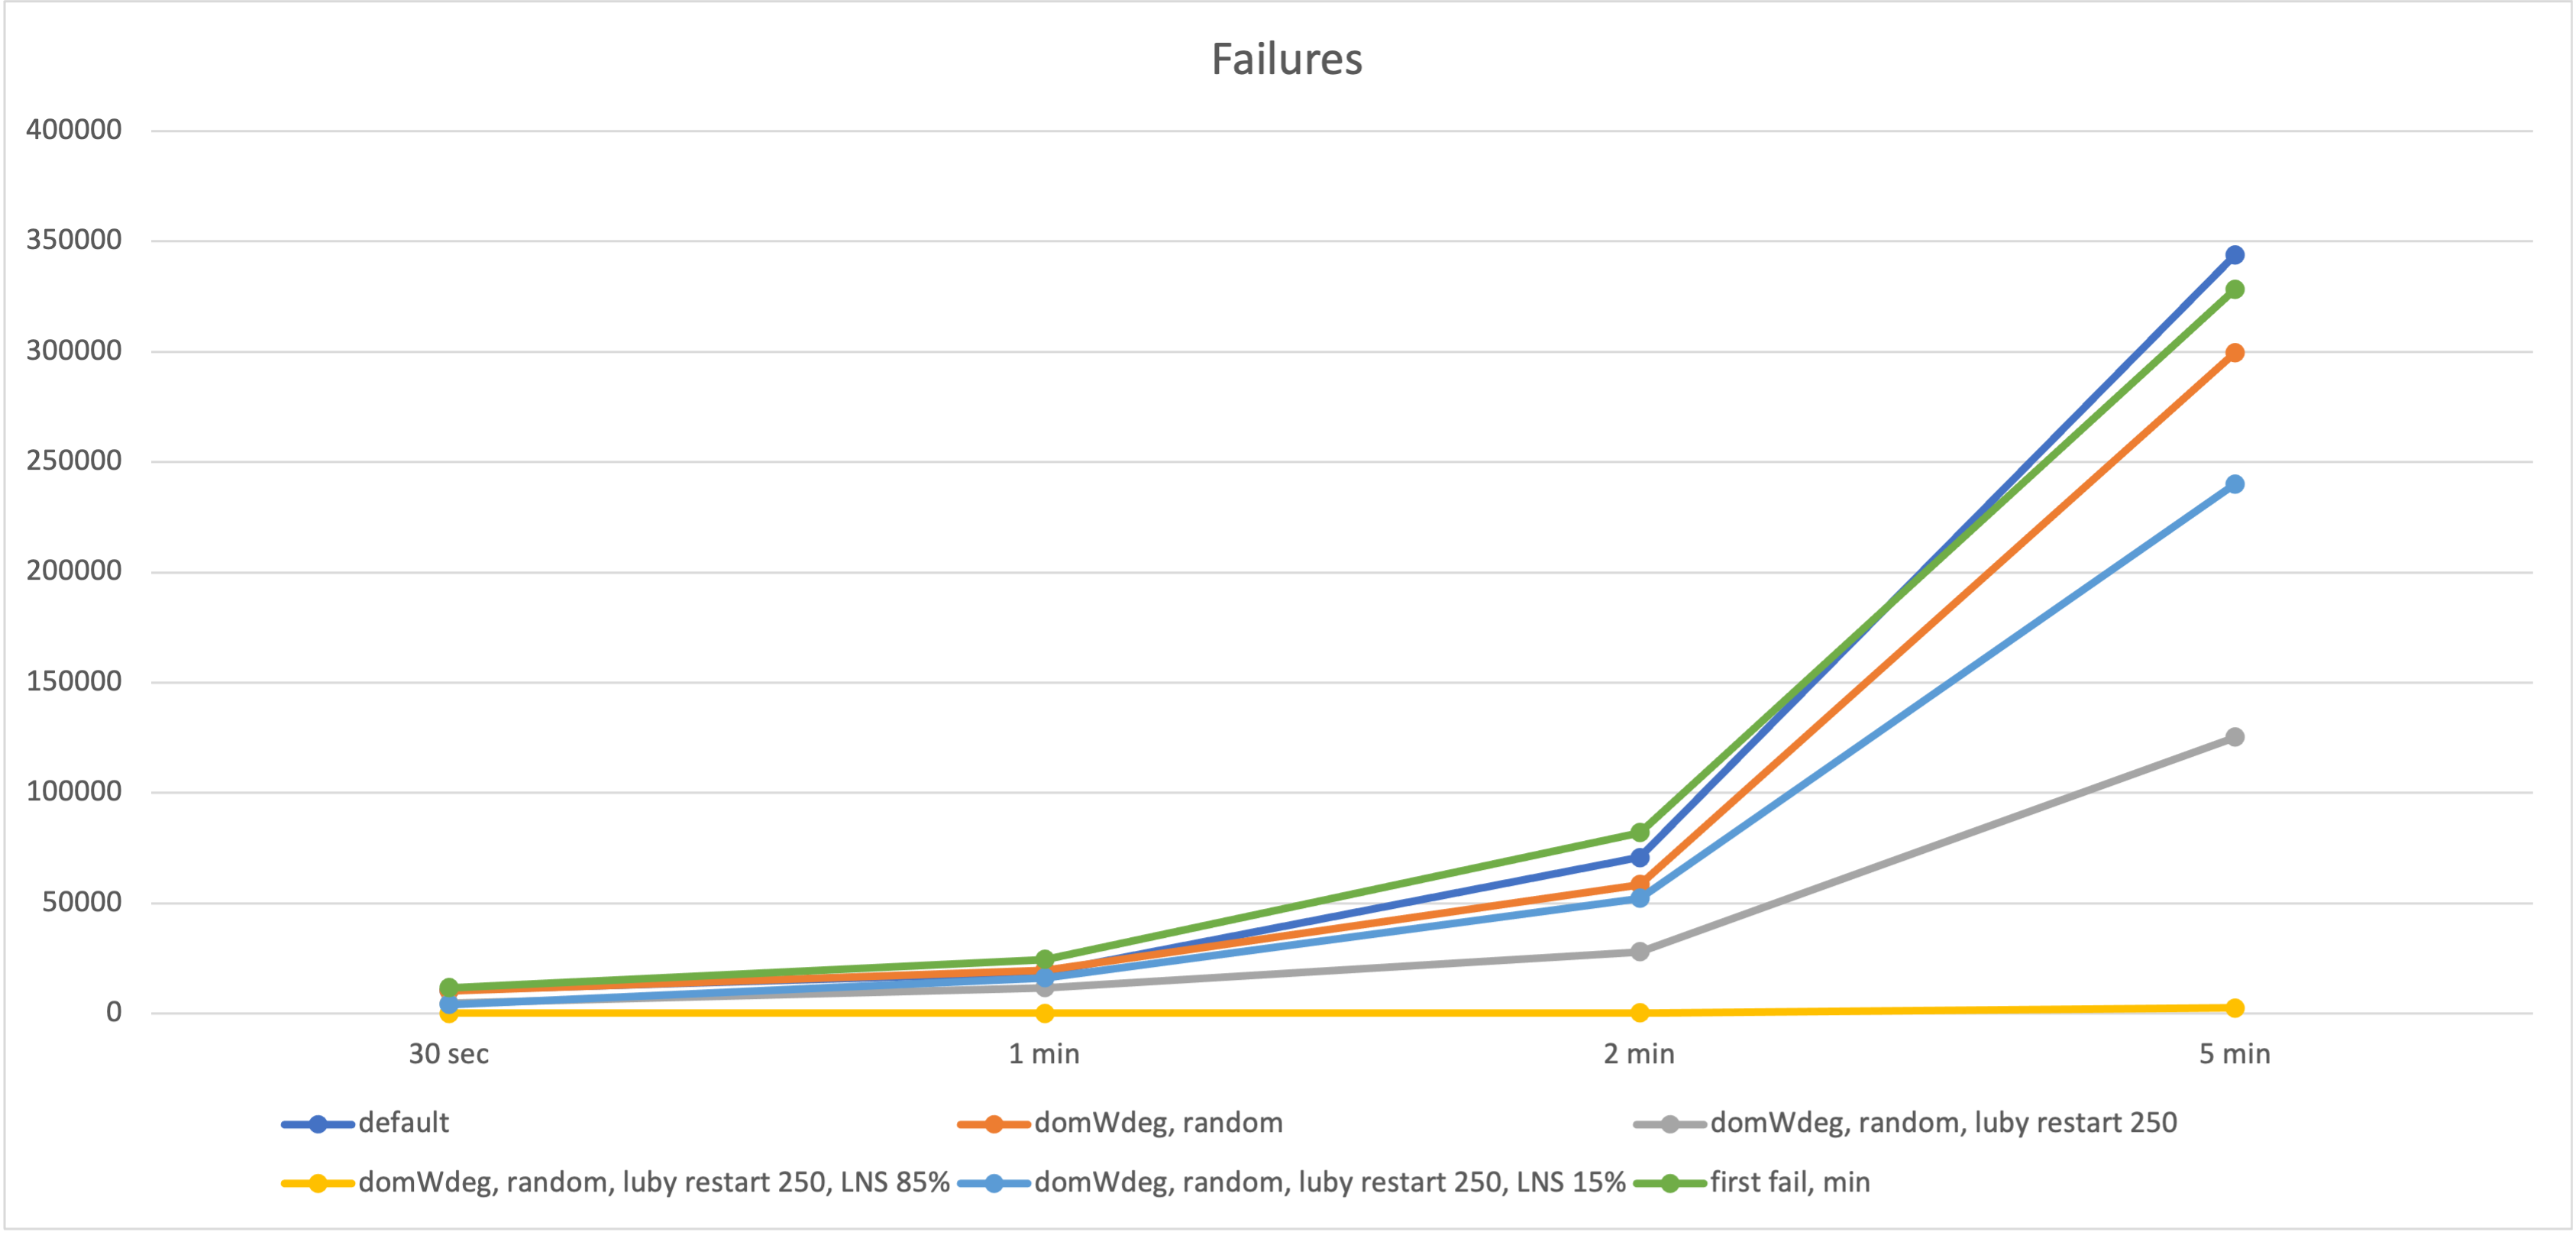
\includegraphics[width=0.8\columnwidth]{../graphs/pr02-failures.png}
    \caption{Failures graph for \textbf{pr02}.}
\end{figure}
{
\renewcommand{\arraystretch}{2}
\begin{longtable}[h]{| c | c | c | c | c |}
    \hline
    \textbf{Objective function} & \multicolumn{3}{c}{Time limit} & \\
    \hline
    \textbf{Search strategy} & \textbf{\textit{30 sec}} & \textbf{\textit{1 min}} & \textbf{\textit{2 min}} & \textbf{\textit{5 min}} \\
    \hline
    \endhead
    default search                                         & 60.927.260 & 59.756.470 & 58.672.370 & 58.613.150 \\
    \hline
    domWdeg, random                                        & 62.665.740 & 61.870.190 & 60.691.370 & 60.429.650 \\
    \hline
    domWdeg, random, Luby restart L=250                    & 61.235.830 & 60.676.010 & 57.212.780 & 57.153.870 \\
    \hline
    \textit{domWdeg, random, Luby restart L=250, LNS 85\%} & 64.350.170 & 61.752.770 & 56.974.800 & 41.023.190 \\
    \hline
    domWdeg, random, Luby restart L=250, LNS 15\%          & 61.523.110 & 58.896.400 & 55.924.200 & 55.417.810 \\
    \hline
    first fail, min                                        & 59.394.090 & 59.700.650 & 59.519.090 & 59.394.090 \\
    \hline
\end{longtable}
}
\begin{figure}[H]
    \centering
    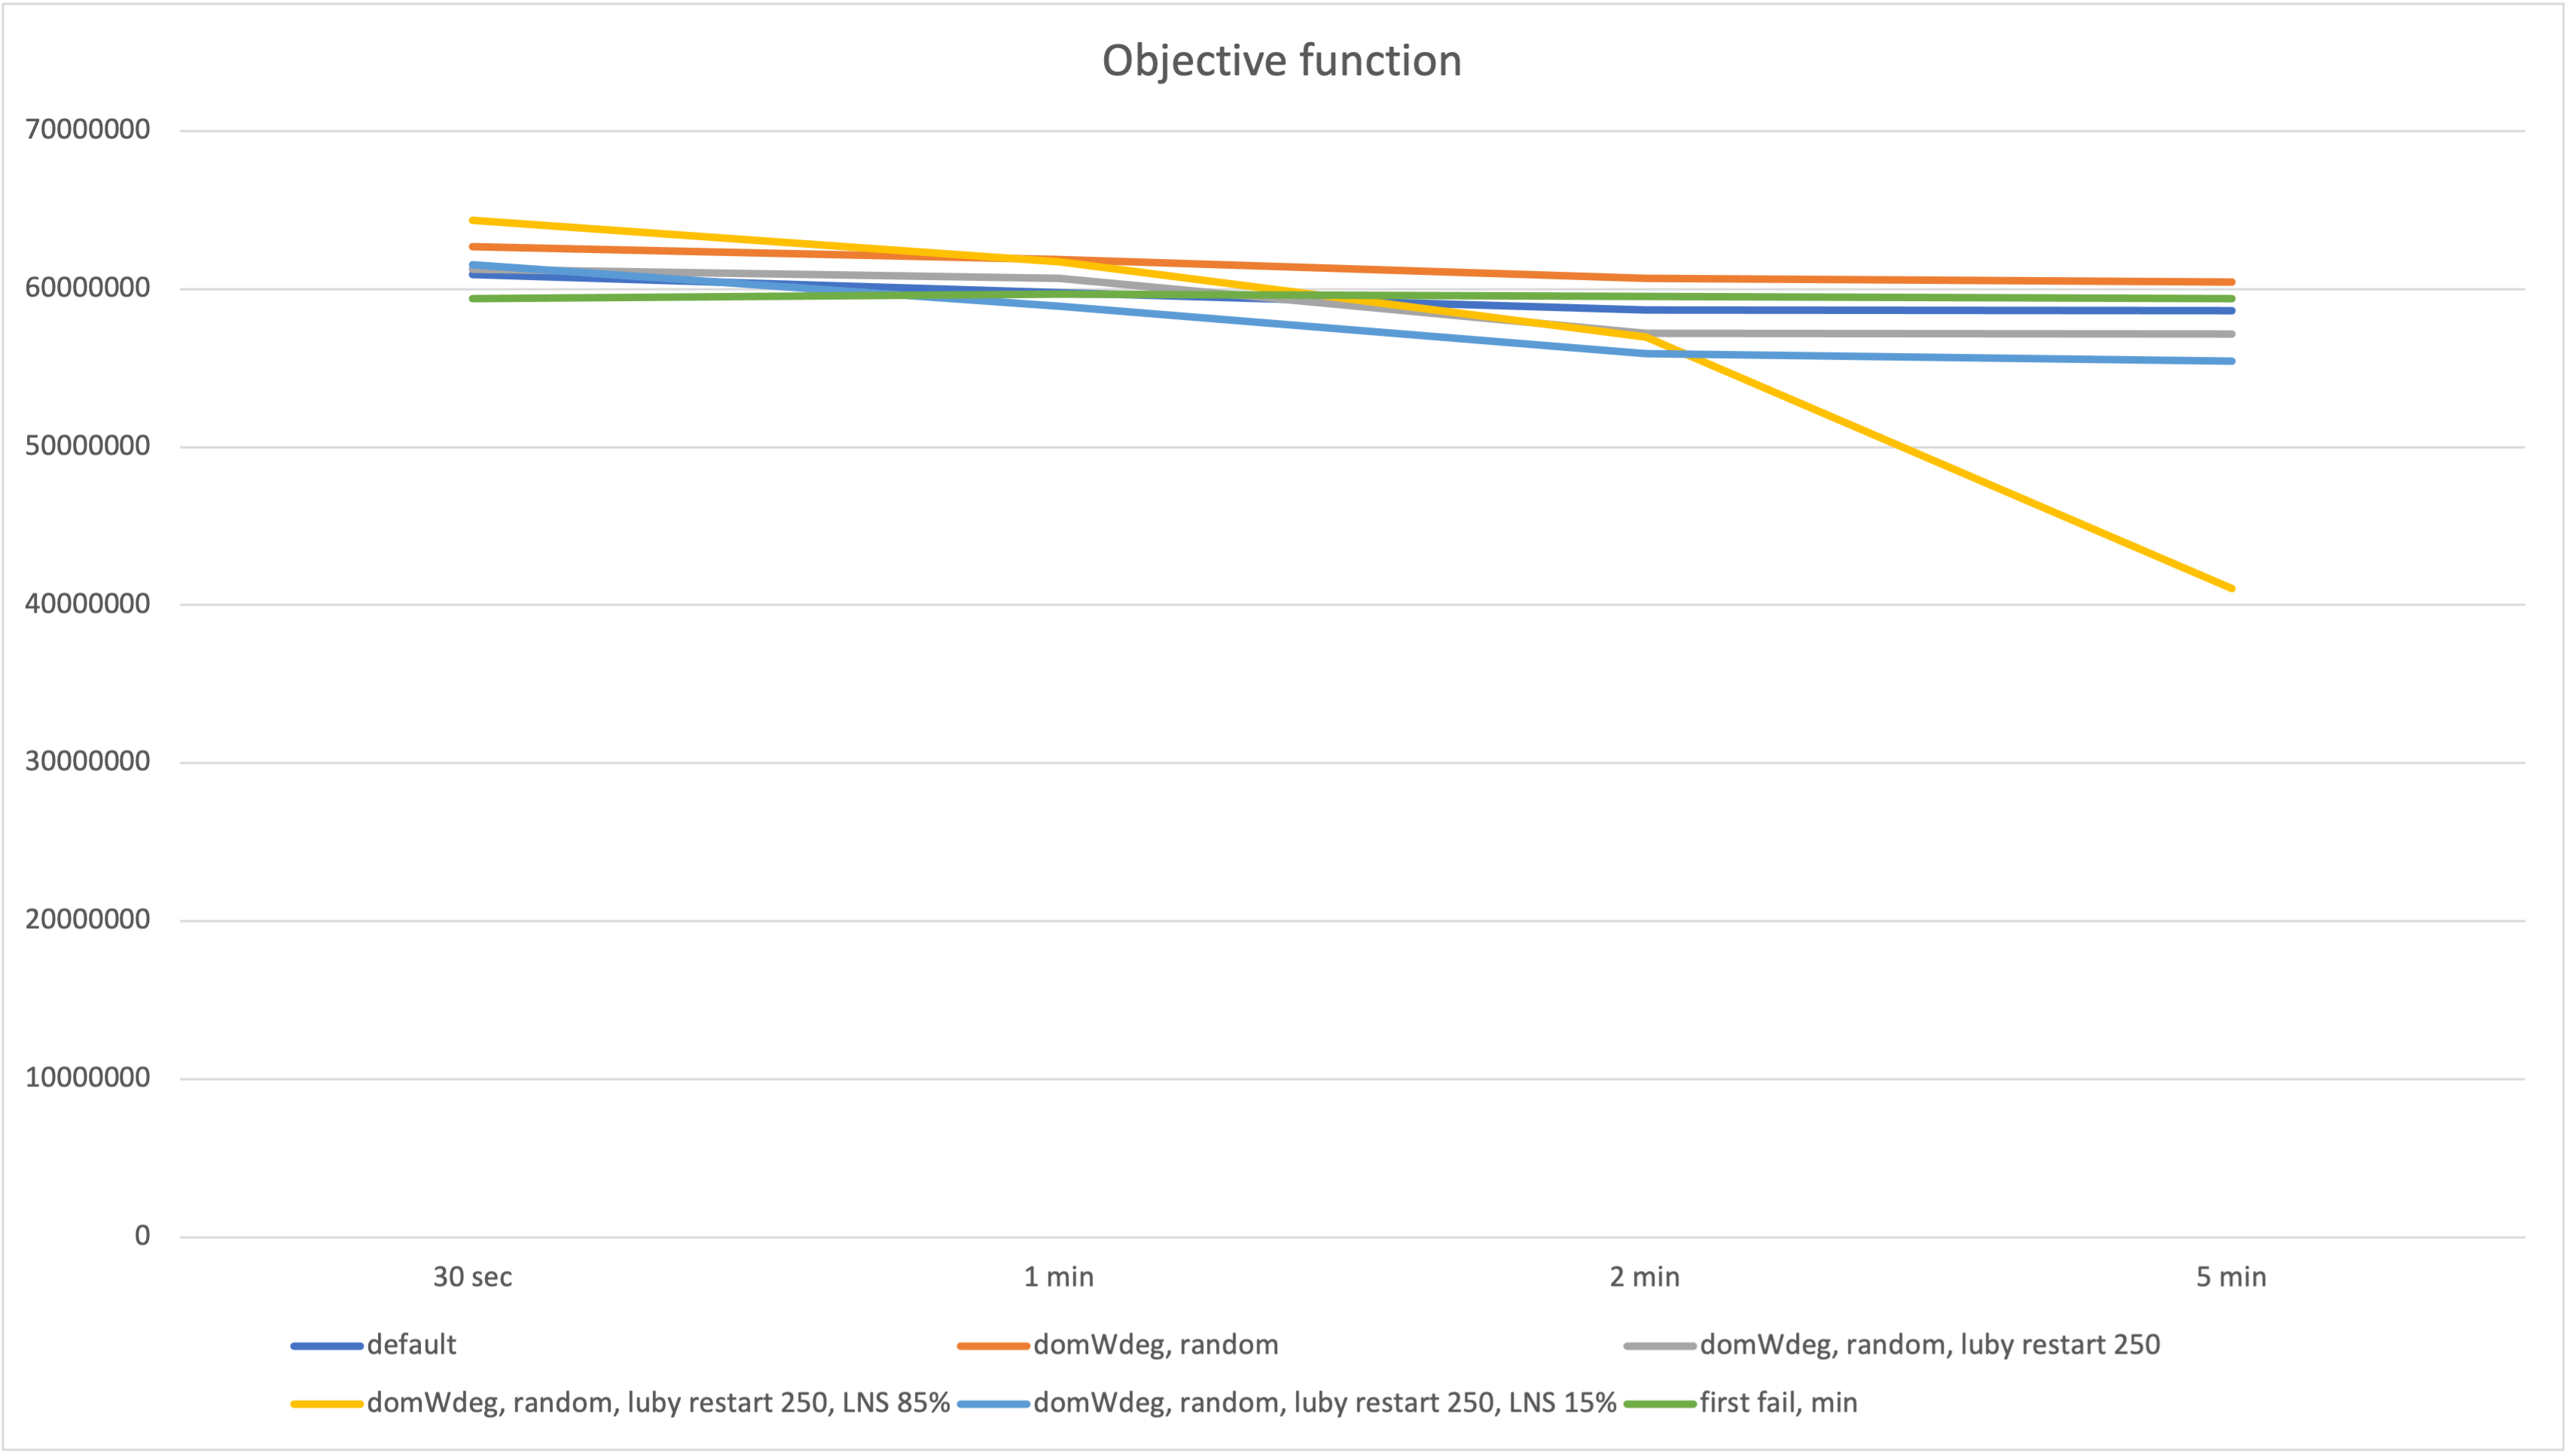
\includegraphics[width=0.8\columnwidth]{../graphs/pr02-objf.png}
    \caption{Objective functions graph for \textbf{pr02}.}
\end{figure}
{
\renewcommand{\arraystretch}{2}
\begin{longtable}[h]{| c | c | c | c |}
    \hline
    \textbf{Weights} & \textbf{Objective function} & \textbf{Total distance} & \textbf{Used vehicles} \\
    \hline
    \endhead
    $\alpha = 10, \beta = 0$ & 36.450.060 & 3.645.006 & 12 \\
    \hline
    $\alpha = 7, \beta = 3$  & 24.636.532 & 3.519.499 & 13 \\
    \hline
    $\alpha = 5, \beta = 5$  & 17.910.480 & 3.582.083 & 13 \\
    \hline
    $\alpha = 3, \beta = 7$  & 10.480.247 & 3.493.390 & 11 \\
    \hline
    $\alpha = 0, \beta = 10$ &         70 & 6.570.642 &  7 \\
    \hline
\end{longtable}
}
\begin{figure}[H]
    \centering
    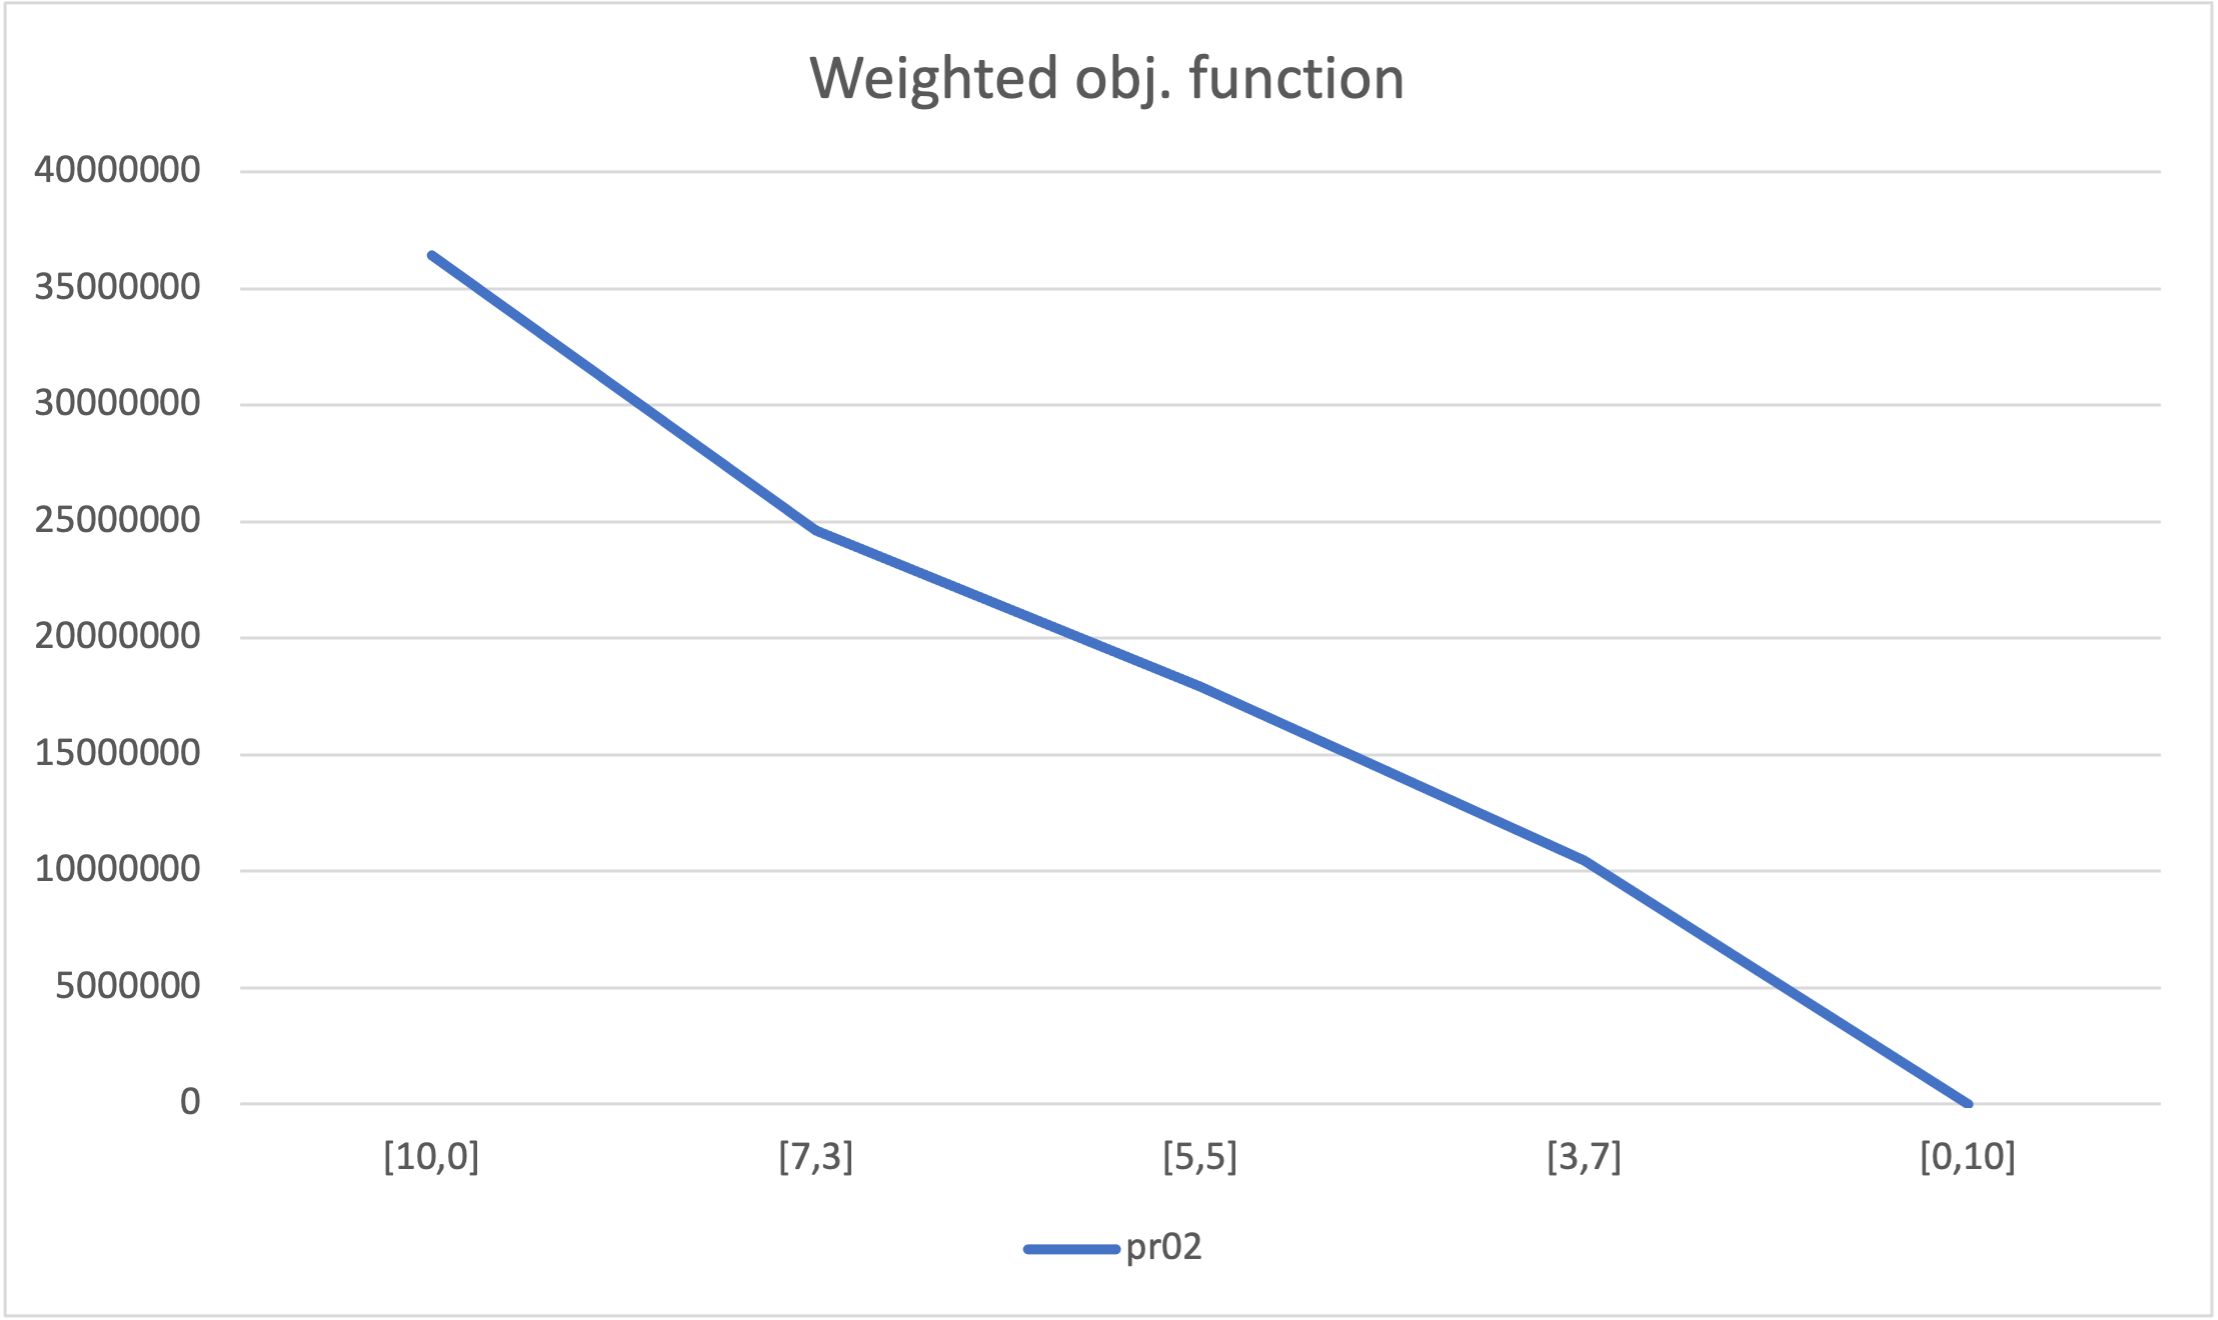
\includegraphics[height=0.25\textheight]{../graphs/pr02-wobjf.png}
    \caption{Weighted objective functions graph for \textbf{pr02}.}
\end{figure}

\begin{figure}[H]
    \centering
    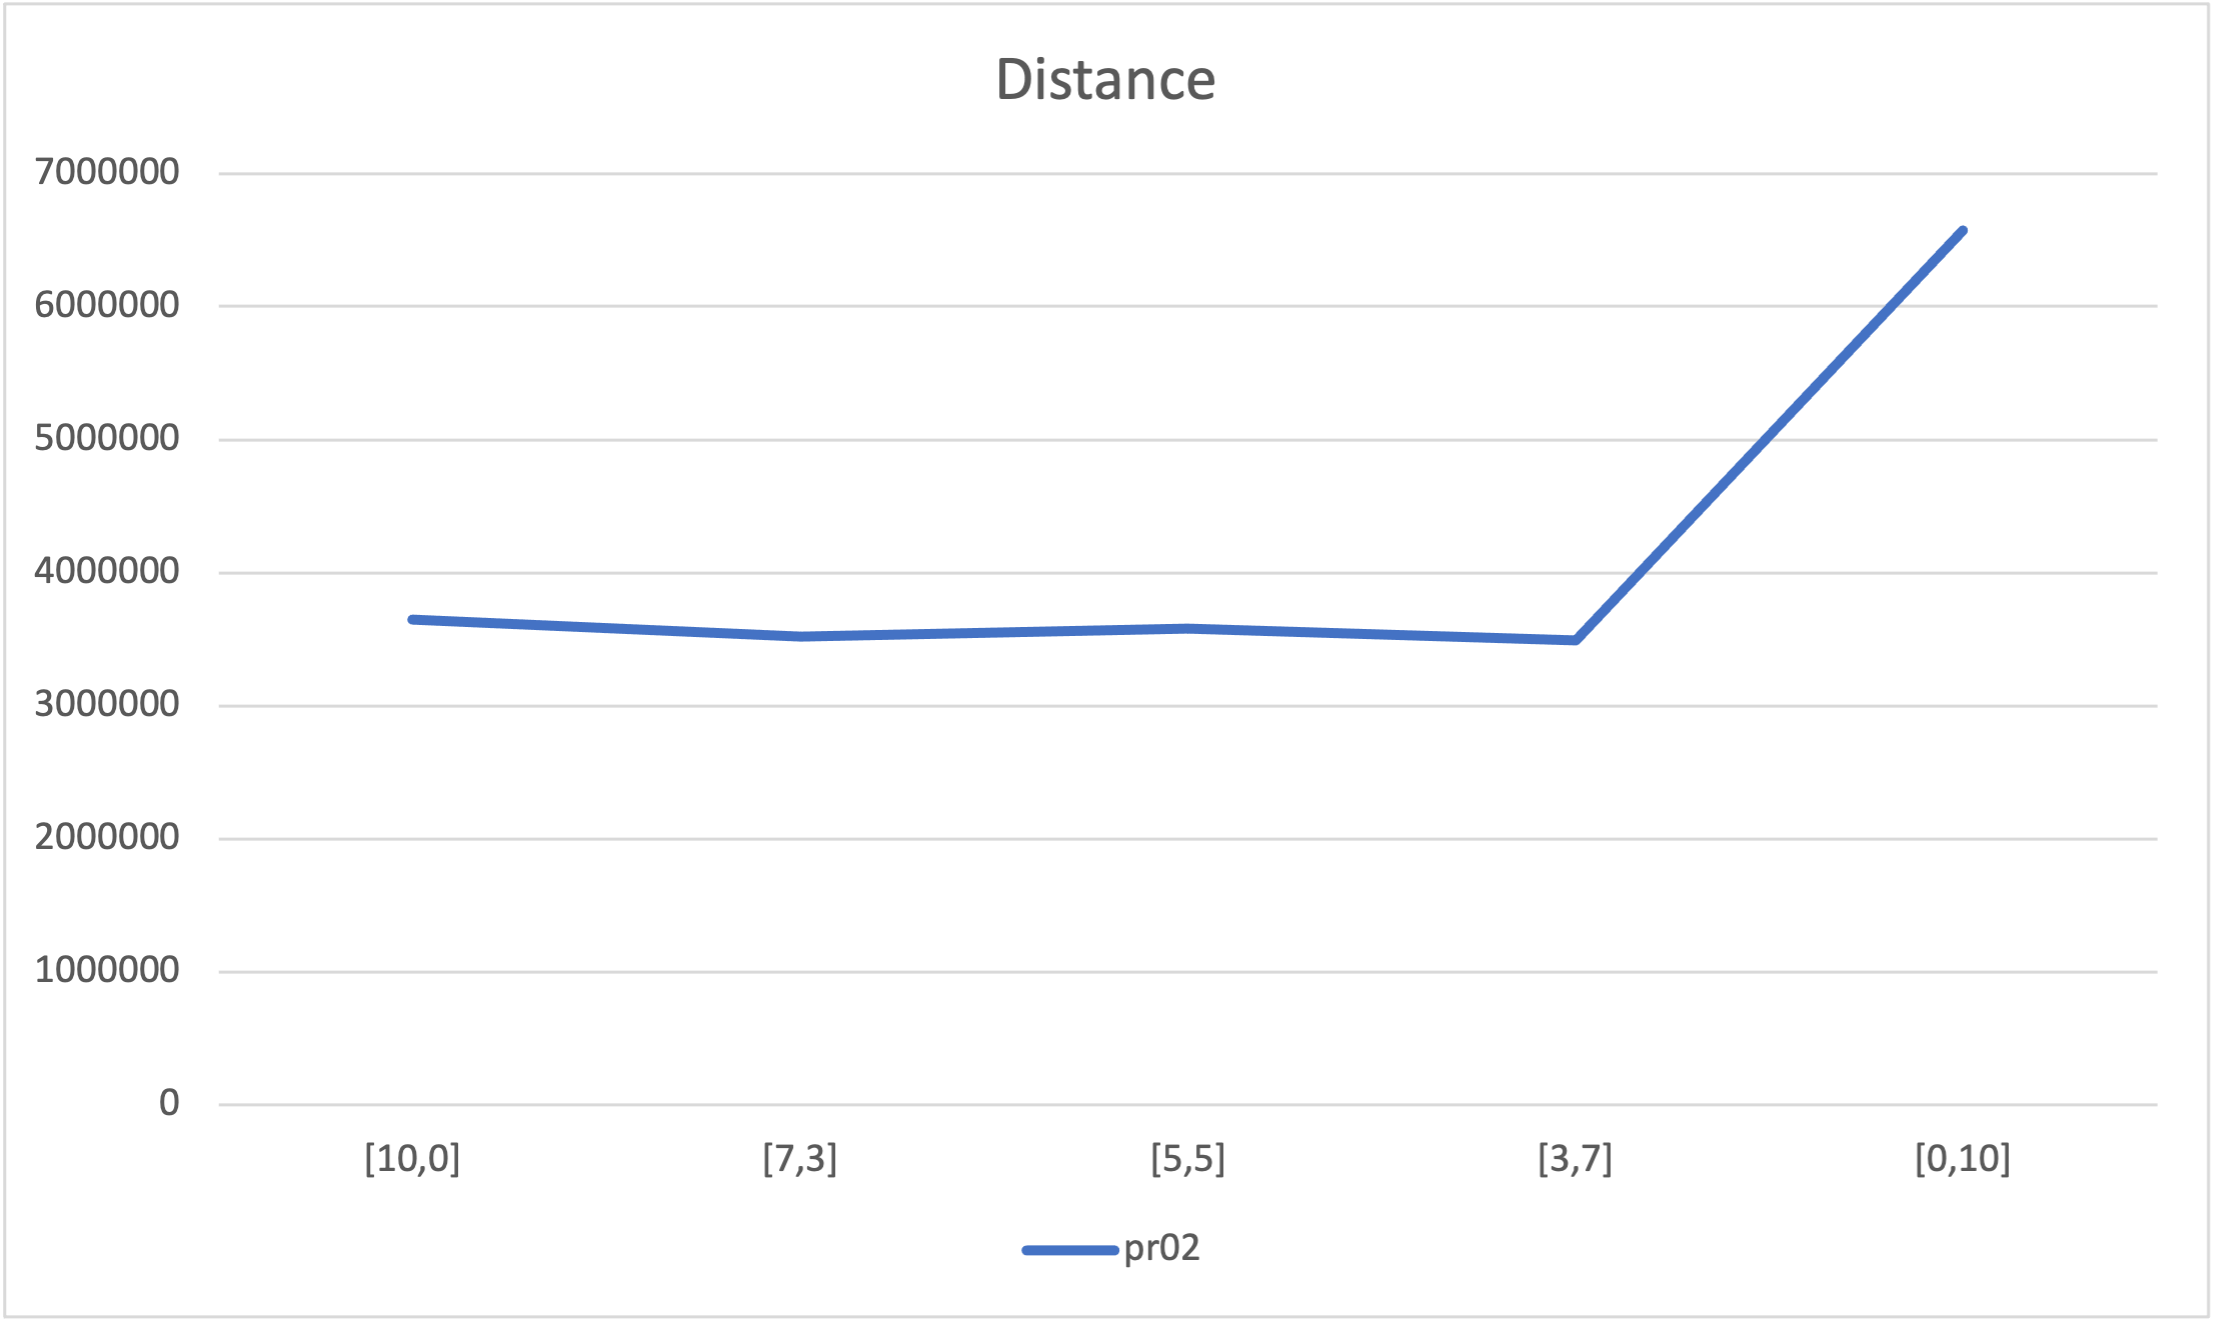
\includegraphics[height=0.25\textheight]{../graphs/pr02-distance.png}
    \caption{Distances graph for \textbf{pr02}.}
\end{figure}

\begin{figure}[H]
    \centering
    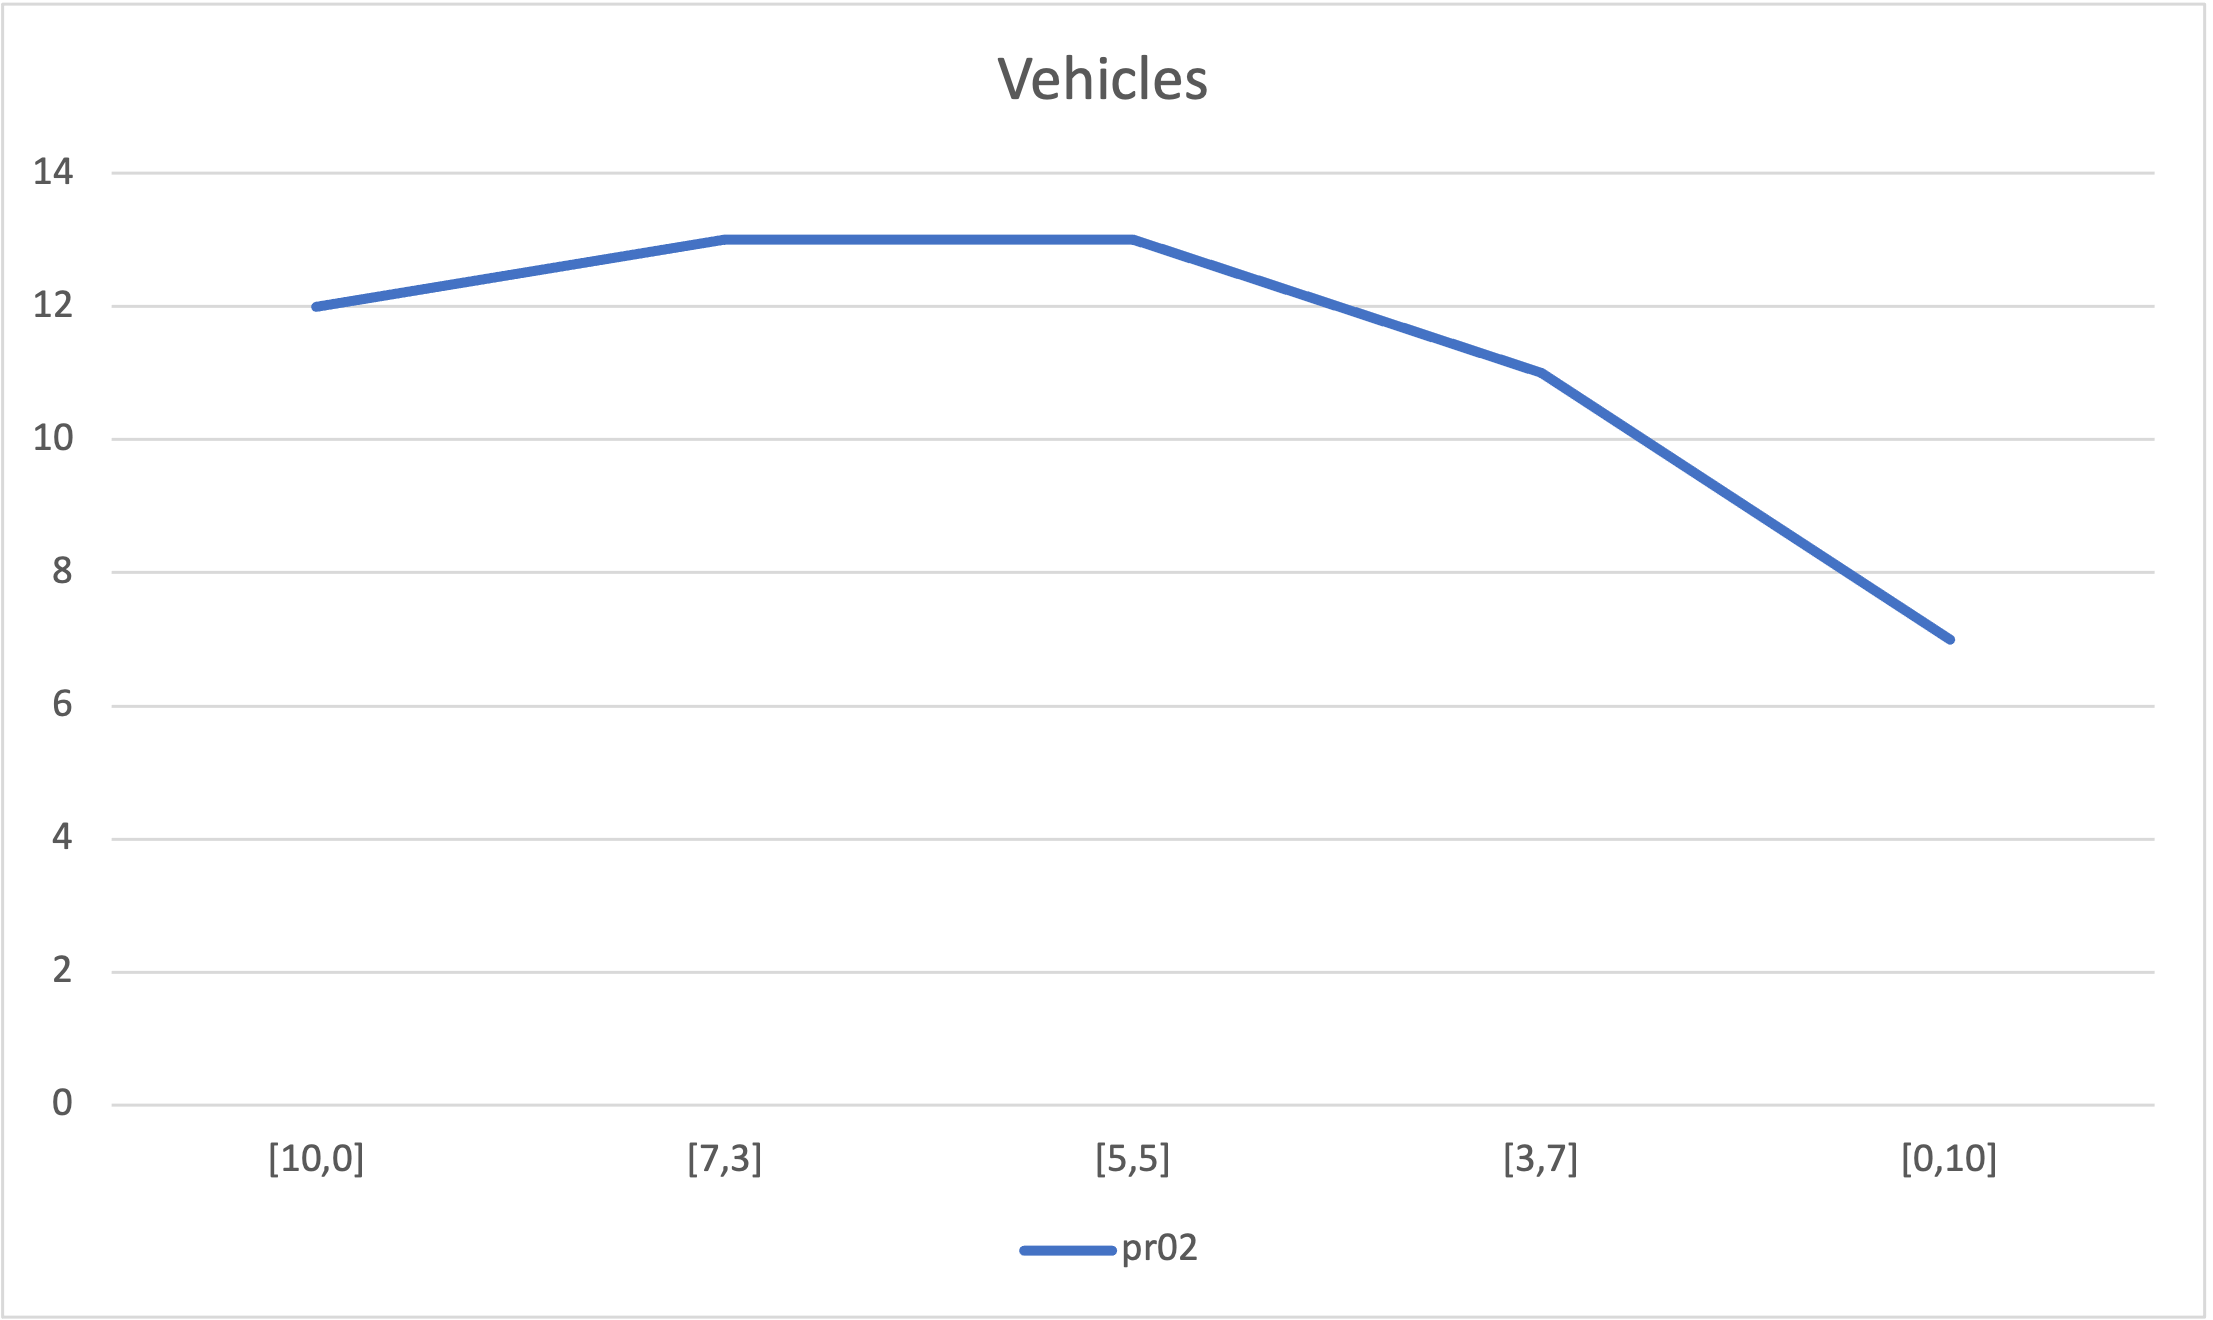
\includegraphics[height=0.25\textheight]{../graphs/pr02-vehicles.png}
    \caption{Vehicles used graph for \textbf{pr02}.}
\end{figure}

\newpage